\subsection{CentralServer}

\textbf{Funktionalitet}\\
Iht. afsnittet "Specifikation og analyse" er hovedfunktionaliteten i CentralServer en TCP/IP socket-server, hvor flere klienter kan forbinde til - og kommunikere med - asynkront. Derudover var det et krav, at CentralServer skulle håndtere alt interaktion med Database.\\

For at imødekomme kravene på fornuftig vis, implementere CentralServer følgende funktionalitet:

\begin{itemize}
	\item Multitrådet programmering.
	\item Et event-baseret beskedsystem, som tillader tråde at sende beskeder til hinanden, samt synkronisering af tråde.
	\item Logging af beskeder i forskellige niveauer samt til forskellige former for outputs.
	\item En socket-server, der altid er klar til at acceptere indkommende forbindelser.
	\item En objektorienteret tilgang til en SQL server.
	\item Håndtering af kommandoer, som er modtaget fra klienter.
\end{itemize}


\textbf{Afhængigheder}\\
CentralServer er afhængig af følgende:

\begin{itemize}
	\item Visual Studio 2015: der benyttes syntax, som ikke er understøttet af C\# compileren i Visual Studio 2013.
	\item Entity Framework: benyttes til at have en objektorienteret tilgang til databasen.
	\item SharedLib: der benyttes datamodeller og funktionalitet til at håndtere dataprotokol.
\end{itemize}


\textbf{Design}\\
Ifm. design af CentralServer er der lagt vægt på følgende:

\begin{itemize}
	\item Mulighed for udvidelse: klasser skal ikke være afhængige af specifikke implementeringer, men skal derimod afhænge af interfaces hvor muligt.
	\item Minimal blokering: tråde skal generelt kun blokere, hvor det er nødvendigt, da blokering er en kostbar operation.
	\item Testbarhed: test af flertrådede programmer, og programmer med databaser, er ikke en del af vores pensum. Der er derfor blevet prioriteret at teste de aspekter af CentralServer, som ikke har med disse discipliner at gøre. Dette har resulteret i begrænsninger ift. både unit- og integrationstesting.
\end{itemize}

\begin{figure}[H]
    \centering
    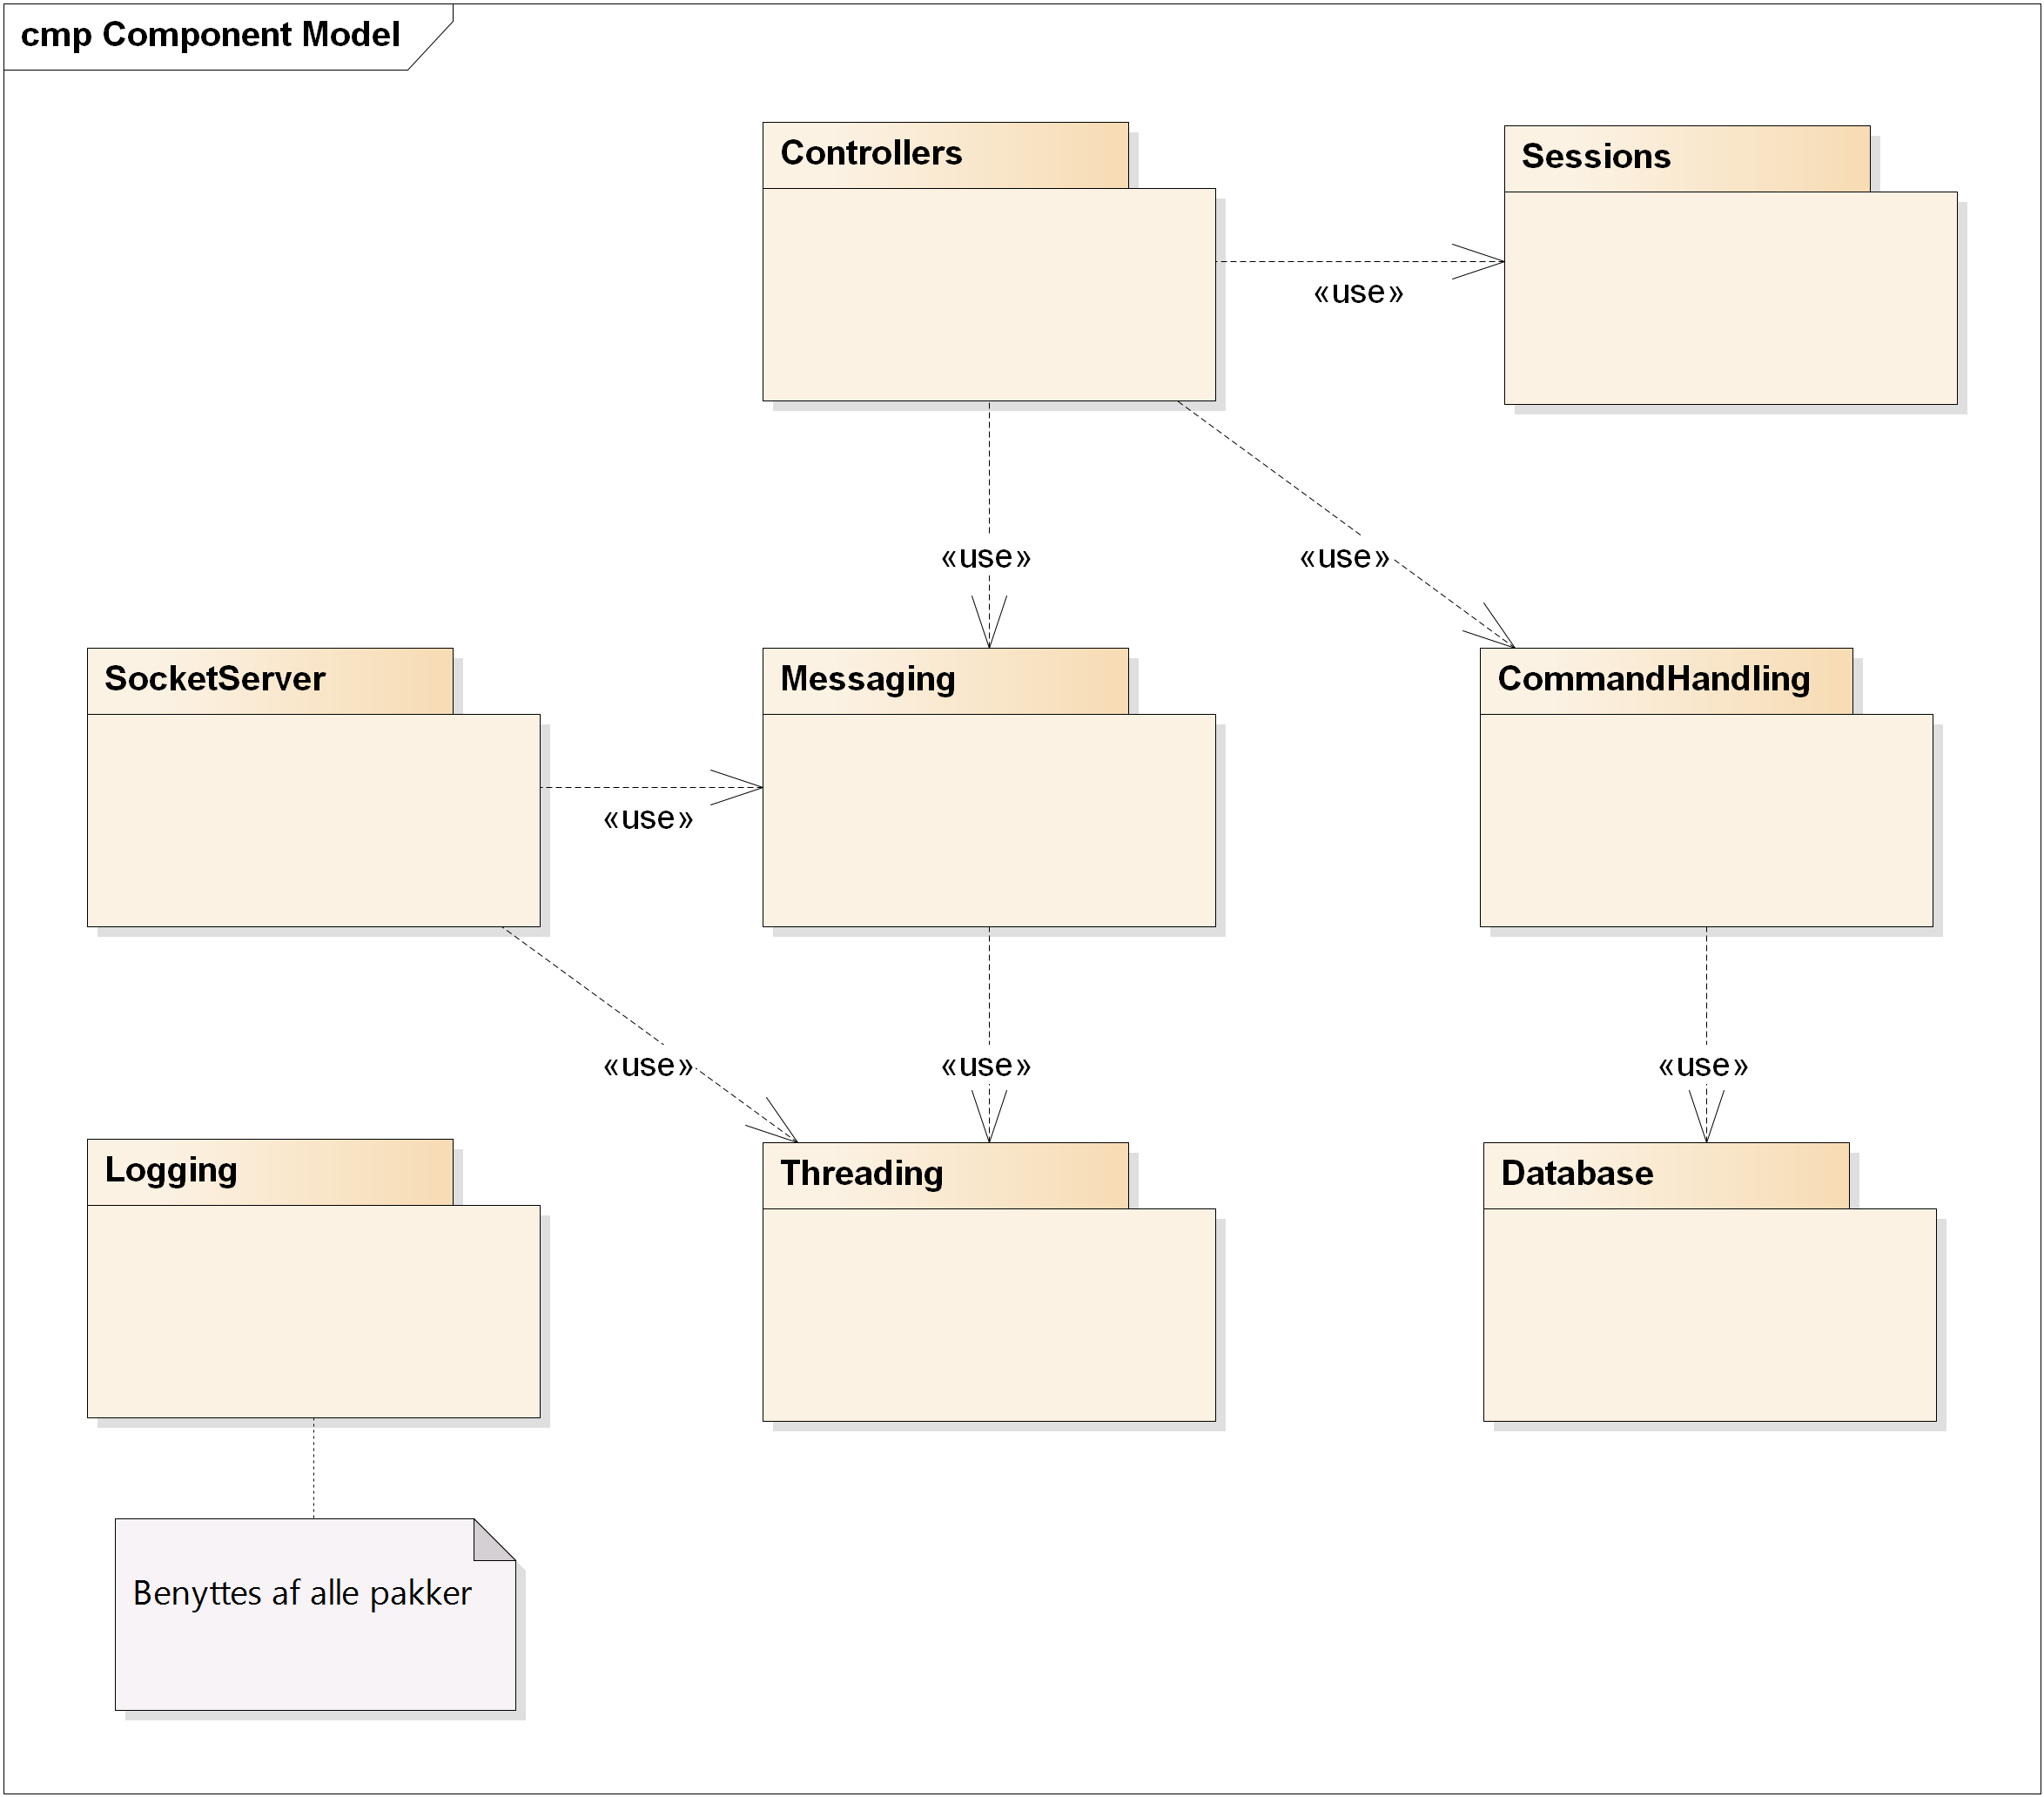
\includegraphics[width=1\textwidth]{../Projektdokumtation/Systemdesign/CentralServer/Images/Packages.png}
    \caption{Pakkediagram for CentralServer}
    \label{fig:CSPackages}
\end{figure}


\textbf{Controllers}\\
Indeholder implementeringerne af de forskellige tråde, der kan modtage beskeder fra andre tråde. Denne pakke benytter følgende pakker:

\begin{itemize}
	\item Sessions: benyttes til at identificere klienter ud fra sessions ID.
	\item Messaging: benyttes til at kunne modtage beskeder fra andre tråde.
	\item CommandHandling: benyttes til at håndtere kommandoer, som er modtaget fra forbundne klienter.
\end{itemize}


\textbf{Sessions}\\
Indeholder funktionalitet til at identificere forbundne klienter ud fra et sessions ID.\\

\textbf{Messaging}\\
Indeholder beskedsystem, som tillader tråde at kommunikere med hinanden. Denne pakke benytter Threading-pakken til at implementere en tråd, der kan modtage beskeder fra andre tråde.\\

\textbf{SocketServer}\\
Indeholder implementeringen af socket-serveren. Denne pakke benytter Threading-pakken til at eksekvere i en tråd, og den benytter Messaging-pakken til at sende beskeder til en controller, når en ny klient er forbundet.\\

\textbf{CommandHandling}\\
Indeholder håndtering af kommandoer, som er modtaget fra forbundne klienter. Det er heri, at business logic er placeret. Denne pakker benytter Database-pakken til at tilgå data fra databasen.\\

\textbf{Threading}\\
Indeholder en hjælpe-klasse samt et interface, som kan benyttes til at starte tråde.\\

\textbf{Logging}\\
Indeholder funktionalitet til at logge begivenheder. Logging benyttes af alle andre pakker.\\

\textbf{Database}\\
Indeholder database access layer (DAL). Her ligger implementering af Entity Framework contexten.